%
% Scott Percic
%
\documentclass[12pt,fullpage]{article}
\usepackage{fullpage}
\usepackage{psfrag}                                          % LaTeX graphics tool
\usepackage{pslatex}                                         % avoids the default cmr font
\usepackage{graphicx}                                        % graphics package 
\usepackage{epsfig}                                          % figures
\usepackage{hyperref}
\usepackage{color}

\begin{document}

\noindent
{\bf Standard normal distribution} (from \color{blue}\url{http://www.math.wm.edu/~leemis/chart/UDR/UDR.html}\color{black})

\noindent
The shorthand $X \sim N(0,1)$ is used to indicate that the random variable $X$ has the standard normal distribution.
A standard normal random variable $X$ has probability density function 
$$
f(x) = \,{\frac {{e^{-x^{\kern 0.04 em 2}/2\,}}}{\sqrt {
2\pi }}}  \qquad \qquad  -\infty < x < \infty .
$$
The standard normal random variable arises because 
a normal random variable with mean $\mu$ and variance $\sigma ^ 2$ can
be standardized by subtracting $\mu$, then dividing by $\sigma$.
This means that only a single table is required for all calculations
involving the normal distribution.
The probability density function is illustrated below.
{\begin{figure}[h!]
\begin{center}
\psfrag{labx}{$x$}
\psfrag{labf}{$f(x)$}
\includegraphics[width=3.2in]{StandardnormalPlot.ps}
\end{center}
\end{figure}}

\noindent
The cumulative distribution function is
$$
F(x) = \frac{1}{2}+\frac{1}{2}\,{{\rm erf}\left(\frac{x}{\sqrt{2}}\right)}\qquad \qquad  -\infty < x < \infty
$$
where
$$
{\rm erf}(x)=\frac{2} {\sqrt{\pi}} \int_{0} ^ {x} e ^ {-t ^ {2}} \, dt \qquad \qquad x > 0,
$$
and ${\rm erf}(-x) = - {\rm erf}(x)$.
The survivor function on the support of $X$ is
$$
S(x) = \frac{1}{2}-\frac{1}{2}\,{{\rm erf}\left(\frac{x}{\sqrt{2}}\right)}\qquad \qquad  -\infty < x < \infty .
$$
The hazard function on the support of $X$ is
$$
h(x) = -{\frac {{{\rm e}^{-\frac{1}{2}\,{x}^{2}}}\sqrt {2}}{\sqrt {\pi }
\left( -1+{{\rm erf}\left(\frac{x}{\sqrt{2}}\right)} \right) }}\qquad \qquad  -\infty < x < \infty .
$$
The cumulative hazard function on the support of $X$ is
$$
H(x) = - \ln S(x) =\ln  \left( 2 \right) -\ln  \left(\kern -0.08 em 1-
{{\rm erf}\left(\frac{x}{\sqrt{2}}\right)}\kern -0.08 em\right) \qquad \qquad  -\infty < x < \infty .
$$
The inverse distribution function of $X$ is
$$
F^{-1}(u)=\sqrt{2}({\rm erf}^{\kern 0.08 em -1}(2u-1)) \qquad \qquad 0\leq u \leq 1.
$$
The median and mode of $X$ are 0.\\
\\
The moment generating function of $X$ is
$$
M(t) = {{\rm e}^{\kern 0.08 em t^2/2}} \qquad \qquad  -\infty < t < \infty .
$$
The characteristic function of $X$ is
$$
\phi(t) = {{\rm e}^{-t^2/2}} \qquad \qquad  -\infty < t < \infty .
$$
The population mean, variance, skewness, and kurtosis of $X$ are
$$
E[X] = 0 \qquad \qquad 
V[X] = 1 \qquad \qquad 
E\left[ \left( \frac{X - \mu}{\sigma} \right) ^ {\kern -0.08 em 3} \right] = 0 \qquad \qquad 
E\left[ \left( \frac{X - \mu}{\sigma} \right) ^ {\kern -0.08 em 4} \right] = 3.
$$


\vspace{0.1in}

\noindent
{\bf APPL verification:}
The APPL statements
\begin{verbatim}
X := StandardNormalRV();
CDF(X);
SF(X);
HF(X);
IDF(X);
Mean(X);
Variance(X);
Skewness(X);
Kurtosis(X);
MGF(X);
\end{verbatim}
verify the cumulative distribution function, survivor function, hazard function, inverse distribution function, population mean, variance, skewness, kurtosis, and moment generating function.

\end{document}
